%Time-stamp: "Last modified: 2018-08-02 10:42:16 (d_yasaki)"
\documentclass[ms, hidelinks]{uncgdissertationexp}
\setcounter{secnumdepth}{1}
% default is 12pt, phd, doublespaced.
% Masters students should use the ma on as shown below.
% \documentclass[ma]{uncgdissertation}




%%------------------------------------------------------------------%%
%%------------------------- Import Packages ------------------------%%
%%------------------------------------------------------------------%%
%% This is where you can put other packages that you may need.
\usepackage[lofdepth,lotdepth,caption=false]{subfig}
\usepackage{fancyhdr}
\usepackage{amsmath, amssymb, graphicx}
\usepackage{xspace}
\usepackage{braket}
\usepackage{color}
\usepackage{setspace}
\usepackage{fancyvrb}
\usepackage{array}
\usepackage{ifxetex,ifluatex}
\usepackage{etoolbox}
\usepackage{booktabs}
\usepackage[table]{xcolor}
\usepackage{tabu}
\usepackage{longtable}
\usepackage{titlesec}
\usepackage{lmodern}
\usepackage{chngcntr}
\usepackage{graphicx}
\counterwithin*{figure}{chapter}
\counterwithin*{table}{chapter}
\usepackage{capt-of} %trying to get figures to work
\usepackage{float}
\usepackage{pdflscape}
\usepackage{microtype, amsfonts, amsthm}
\usepackage[colorlinks=false]{hyperref}
\pdfstringdefDisableCommands{\let\MakeUppercase\relax}
%\usepackage{showframe}
%useful package to ensure margins are correct.

\usepackage[document]{ragged2e} %left justify
\setlength{\RaggedRightRightskip}{0pt plus 4em}
\usepackage[all]{nowidow} % to make sure no single lines appear at the bottom or top of the page 

\usepackage[utf8]{inputenc} %I need the mu symbol and others
\usepackage{textcomp}
% fix for pandoc 1.14
\providecommand{\tightlist}{
  \setlength{\itemsep}{0pt}\setlength{\parskip}{0pt}}

\def\tightlist{} 
%%tightlist error

%
% commands and environments needed by pandoc snippets
% extracted from the output of `pandoc -s`
%% Make R markdown code chunks work

\ifxetex
  \usepackage{fontspec,xltxtra,xunicode}
  \defaultfontfeatures{Mapping=tex-text,Scale=MatchLowercase}
\else
  \ifluatex
    \usepackage{fontspec}
    \defaultfontfeatures{Mapping=tex-text,Scale=MatchLowercase}
  \else
    \usepackage[utf8]{inputenc}
  \fi
\fi
\usepackage{color}
\usepackage{fancyvrb}
\DefineShortVerb[commandchars=\\\{\}]{\|}
\DefineVerbatimEnvironment{Highlighting}{Verbatim}{commandchars=\\\{\}}
% Add ',fontsize=\small' for more characters per line
% \newenvironment{Shaded}{}{}
% \newcommand{\KeywordTok}[1]{\textcolor[rgb]{0.00,0.44,0.13}{\textbf{{#1}}}}
% \newcommand{\DataTypeTok}[1]{\textcolor[rgb]{0.56,0.13,0.00}{{#1}}}
% \newcommand{\DecValTok}[1]{\textcolor[rgb]{0.25,0.63,0.44}{{#1}}}
% \newcommand{\BaseNTok}[1]{\textcolor[rgb]{0.25,0.63,0.44}{{#1}}}
% \newcommand{\FloatTok}[1]{\textcolor[rgb]{0.25,0.63,0.44}{{#1}}}
% \newcommand{\CharTok}[1]{\textcolor[rgb]{0.25,0.44,0.63}{{#1}}}
% \newcommand{\StringTok}[1]{\textcolor[rgb]{0.25,0.44,0.63}{{#1}}}
% \newcommand{\CommentTok}[1]{\textcolor[rgb]{0.38,0.63,0.69}{\textit{{#1}}}}
% \newcommand{\OtherTok}[1]{\textcolor[rgb]{0.00,0.44,0.13}{{#1}}}
% \newcommand{\AlertTok}[1]{\textcolor[rgb]{1.00,0.00,0.00}{\textbf{{#1}}}}
% \newcommand{\FunctionTok}[1]{\textcolor[rgb]{0.02,0.16,0.49}{{#1}}}
% \newcommand{\RegionMarkerTok}[1]{{#1}}
% \newcommand{\ErrorTok}[1]{\textcolor[rgb]{1.00,0.00,0.00}{\textbf{{#1}}}}
% \newcommand{\NormalTok}[1]{{#1}}
% \newcommand{\OperatorTok}[1]{\textcolor[rgb]{0.00,0.44,0.13}{\textbf{{#1}}}}
% \newcommand{\BuiltInTok}[1]{\textcolor[rgb]{0.00,0.44,0.13}{\textbf{{#1}}}}
% \newcommand{\ControlFlowTok}[1]{\textcolor[rgb]{0.00,0.44,0.13}{\textbf{{#1}}}}





%%------------------------------------------------------------------%%
%%--------------------------- Content ------------------------------%%
%%------------------------------------------------------------------%%
%% Members of committee.  Guidelines say don't use Dr.
%% Masters students are required to have chair plus two
%% PhD students require chair plus three.
%% The class can handle up to chair plus five.
\chair{Parke Rublee}
\member{Anne Hershey}
\member{Martin Tsui}
%%\member{}

%% Your name goes here.
%% \student{Firstname}{Lastname}
%% Some other options
%%\student{Joe Michael}{Schmoe}  % a full middle name
\student{Ashley S.}{Williams}       % a middle initial

%% Thesis Title
%%    +  Capitalize first letter of important words.
%%    +  Use inverted pyramid shape if title spans more than one line.
%%  Note: You can force break the title onto multiple lines using
%%  \break instead of \\.
\title{Detecting a Microbial Response in Sediment of the Dan River Following a Coal Ash Spill}

%% Degree year.
\degreeyear{2019}


%%------------------------------------------------------------------%%
%%----------------------- Personal Macros --------------------------%%
%%------------------------------------------------------------------%%
%% A central location to add your favorite macros.  A few examples are
%% given below.  See tips for samples.

%% In order to get singlespacing, uncomment the line below.
%\renewcommand{\doublespacing}{\singlespacing}

%% Theorem, Lemma, etc. environments.  You can rename if you wish.
% Theorem style and numbering convention
\theoremstyle{plain}
\newtheorem{theorem}{Theorem}[chapter]
\newtheorem{lemma}[theorem]{Lemma}
\newtheorem{proposition}[theorem]{Proposition}
\newtheorem{conjecture}[theorem]{Conjecture}
\newtheorem{corollary}[theorem]{Corollary}
\newtheorem{algorithm}[theorem]{Algorithm}

% Definition type object style and numbering convention
\theoremstyle{definition}
\newtheorem{definition}[theorem]{Definition}
\newtheorem{example}[theorem]{Example}

% Remark type object style and numbering
\theoremstyle{remark}
\newtheorem*{remark}{Remark}  % the star makes them not numbered
\newtheorem*{notation}{Notation}
\newcommand{\titlecaption}[2]{\caption[#1]{#1. #2}}

%% Other macros
\newcommand{\ZZ}{\mathbb{Z}}  % Integers
\newcommand{\XX}{\mathfrak{X}}

\bibliography{references}

%%------------------------------------------------------------------%%
\begin{document}
\frontmatter      % required

%%------------------------------------------------------------------%%
%% -------------------------- Abstract -----------------------------%%
%%------------------------------------------------------------------%%
\begin{abstract}
Coal ash is the residual material of coal combustion for electricity generation. It contains heavy metals and other pollutants and is generally deposited into reservoir ponds for storage, although it may spill or leach into nearby water and possibly disrupt aquatic communities. In February of 2014, a coal ash spill occurred in the Dan River in Eden, NC. Coal ash contains constituents that may stimulate the growth of mercury methylating bacteria. This study aimed to determine if a microbial response is detectable 1.5 years following the spill using qPCR. We tested three primers targeting mercury methylation. We detected an elevated signal 0.5 km downstream from the spill site relative to some other upstream and downstream locations. However, the highest abundance of amplified targets was observed in the furthest upstream site. We also undertook a survey of bacteria present in a coal ash sample from the coal ash pond that was the source of the spill, located at the retired Dan River Steam Station in Eden, NC. SSU rDNA extracted from 31 isolated organisms was sequenced and the organisms identified to genus level. The community was predominantly composed of \emph{Bacillus} and \emph{Arthrobacter} spp. 14 Isolates were grown in 50\% nutrient broth amended with heavy metals commonly found in coal ash waste (As, Cd, Cr, Hg, Pb, Se, Zn) at environmentally relevant concentrations to characterize their metal tolerance. Growth of coal ash isolates was compared to two isolates cultured from coal ash-free soil. Overall, coal ash isolates exhibited metal tolerance, but so did the soil isolates.
\end{abstract}
%%------------------------------------------------------------------%%
%%---------------------------- Title page --------------------------%%
%%------------------------------------------------------------------%%
%% The title page is required.
\maketitlepage

%%------------------------------------------------------------------%%
%% ------------------------ Copyright page -------------------------%%
%%------------------------------------------------------------------%%
%% This page is required if you opt for a copyright.  Otherwise, don't
% include it.  To omit, just comment out the line below.
%\makecopyrightpage

%%------------------------------------------------------------------%%
%%---------------------------- Dedication --------------------------%%
%%------------------------------------------------------------------%%
\begin{dedication}
  To my love, my kids, and my family.
\end{dedication}
%%------------------------------------------------------------------%%
%%------------------------ Approval page  --------------------------%%
%%------------------------------------------------------------------%%
%% The approval page is required.  If all of your infomation is entered
%% correctly in the contents section, this should come out correctly.
\makeapprovalpage

%%------------------------------------------------------------------%%
%%-------------------------- Acknowledgements ----------------------%%
%%------------------------------------------------------------------%%
%% The acknowledgements are optional but highly recommended.  See tips
%% for details.
\begin{acknowledgments}
\setlength{\parindent}{0.5in}
  I sincerely appreciate the continuous encouragement and guidance from my advisor and mentor Dr.~Parke Rublee, and from my committee members, Drs. Anne Hershey and Martin Tsui. I thank Brian Williams of the Dan River Basin Association for his help and guidance on the river. I also thank Kimber Corson, Matthew Monteverde, and Peija Ku for their assistance during field sampling, as well as Jacob Cleary and our lab mates for their assistance in the lab, including many late night assay reads. A very special thanks to Louisa Liberman for her editorial support and, along with John Rice, Jennifer Petitte, and Leah Blasiak for their copious amounts of encouragement and support. Duke Energy provided access to their boat launch at the spill site. This work was funded by a North Carolina Water Resources Research Institute grant and the UNCG Department of Biology.
\end{acknowledgments}
%%------------------------------------------------------------------%%
%%----------------------------- Preface ----------------------------%%
%%------------------------------------------------------------------%%
%% The preface is optional.
%%\begin{preface}
%%A preface is a statement that either explains the author's
%%reasons for pursuing this subject matter or provides a personal
%%comment about the subject that would not otherwise be included in
%%the document.
%%\end{preface}


%%------------------------------------------------------------------%%
%%---------------------- Table of Contents -------------------------%%
%%------------------------------------------------------------------%%
%% The table of contents is required.
\tableofcontents

%%------------------------------------------------------------------%%
%%---------------------- List of Tables ----------------------------%%
%%------------------------------------------------------------------%%
% Recommended if you have tables.  Comment out if you don't have
% tables.

  \listoftables
  

%%------------------------------------------------------------------%%
%%---------------------- List of Figures ---------------------------%%
%%------------------------------------------------------------------%%
% Recommended if you have figures.  Comment out if you don't have
% figures.

\listoffigures


%%------------------------------------------------------------------%%
%% This signifies that you are done with the frontmatter and ready to
%% proceed to the main part.  The rest of your document goes below.
\mainmatter % required
%%------------------------------------------------------------------%%
\setlength{\parindent}{0.5in}

\hypertarget{intro}{%
\chapter{Introduction}\label{intro}}

Coal is the second most used fuel for electricity generation in the United States. In 2017, approximately 30\% of all electricity production was fueled by coal combustion (Energy Information Administration, 2018). Although the percentage has fallen in recent years due to retirement of coal-fired plants and increases in natural gas and other energy sources, coal remains a main fuel for electricity. Coal combustion results in the production of the waste material, coal ash.

Coal ash is composed of fly ash, bottom ash, and flue gas desulfurized gypsum. Fly ash is a fine powdery substance, comprised primarily of silica that is exhausted through the smokestack. It is produced during the combustion of finely ground coal and most is captured from the exhaust process using electrostatics and scrubber systems. Bottom ash is formed during the combustion of pulverized coal in boilers. It ranges in size from fine sand to fine gravel and is grey to black in color. Bottom ash is too large to be carried up the exhaust system and is collected in an ash hopper. Flue gas desulfurized gypsum is not a direct product of coal combustion, but a product of the scrubber system to remove SO\textsubscript{2} emissions from exhaust (Kisku \emph{et al.}, 2018; Messinger and Silman, 2016).

Physical and chemical properties of coal ash are determined by the geographical location where the raw coal was mined, the type of boiler, and the operating conditions of the power plant (Jayaranjan \emph{et al.}, 2014). Fly ash is composed mainly of oxides such as \(\mathrm{SiO_2}\), \(\mathrm{Al_2O}\), \(\mathrm{Fe_2O}\), \(\mathrm{TiO_2}\), and \(\mathrm{CaO}\). All natural elements can be found in coal ash, and trace elements include, As, Cd, Cr, Hg, Pb, Se, and Zn (Greely Jr. \emph{et al.}, 2014; Jayaranjan \emph{et al.}, 2014; Shaheen \emph{et al.}, 2014). Coal bottom ash consists of silicate, carbonate, aluminate, ferrous materials, and several heavy metals and metalloids. Like fly ash, the chemical composition of the bottom ash is dependent on the source of the raw coal, boiler type, and the refinement process of the raw coal (Jayaranjan \emph{et al.}, 2014).

Once produced and collected, coal ash, in many cases, is mixed with water to form a slurry and stored wet in settling ponds. These ponds are constructed either lined or unlined; open to the atmosphere or capped. The coal ash storage pond located at the Dan River Steam Station, was an open, unlined two-pond system where, the coal ash was pumped into one pond where it settled out of the water column, then pumped to a second pond for further settling before liquid effluent was discharged into the river (Messinger and Silman, 2016). In the US, of the approximately 120 Mt of coal ash is produced annually, 54\% is disposed of in landfills or settling ponds (American Coal Ash Association, 2012). Possible catastrophic impoundment failures and chronic leaching from unlined impoundments allow the mobilization of coal ash including their associated heavy metals into the environment where these metals may enter the food web directly or indirectly through microbially-mediated transformations (Cabral \emph{et al.}, 2016; Deonarine \emph{et al.}, 2013; Hershey \emph{et al.}, 2016; Otter \emph{et al.}, 2012).

On February 2, 2014, two storm water drainage pipes located under a coal ash impoundment pond at the Duke Energy Dan River Steam Station near Eden, NC collapsed, releasing approximately 28,000 cubic yards of coal ash and about 27 million gallons of untreated ash wastewater into the Dan River (Lemly, 2015). Following the spill, water and sediment was sampled from the river and Kerr Reservoir downstream of the spill to assess water quality and human health concerns. Test results showed no constituents to be at levels exceeding safe limits in the water column (Hesterberg \emph{et al.}, 2014; US EPA, 2014). Duke Energy dredged ash deposits at two locations along the river, but likely over 90\% of the ash remains buried in river sediments or has been deposited into Kerr Lake (NC DEQ, 2014). While the test results were encouraging for immediate water quality, the long-term concern is the effect of mobilization of coal ash constituents into the riverine food webs.

\hypertarget{pcr}{%
\chapter{RESPONSE OF MERCURY METHYLATING BACTERIA TO THE COAL ASH SPILL IN THE DAN RIVER}\label{pcr}}

\hypertarget{introduction}{%
\section{Introduction}\label{introduction}}

The February 2014 coal ash spill mobilized coal ash into the Dan River. One constituent of particular concern during leaching and/or impoundment failure is mercury. Inorganic mercury often passes through an organism, but the bioavailable form of mercury, methylmercury (MeHg) is a known neurotoxin and potential endocrine disruptor and has a high affinity for sulfhydryl groups in proteins (Boyd and Barkay, 2012). This may destabilize proteins and lead to decreased enzymatic activity and reduced overall fitness of organisms (Driscoll \emph{et al.}, 2013; Ehrlich and Newman, 2008).

MeHg is produced in anaerobic conditions predominately by sulfate reducing bacteria (SRB), iron reducing bacteria (FeRB), and methanogens (Liu \emph{et al.}, 2014). Coal ash may provide the necessary substrates to stimulate the microbial methylation of Hg (Deonarine \emph{et al.}, 2013). Microorganisms have developed various mechanisms to mitigate effects of high concentrations of heavy metal toxins, such as Hg. These include reduction of the metal to a less toxic form, metal complexation, efflux pumps via an energy-dependent membrane transporter, and extracellular sequestration (Binkley and Simpson, 2003; Poulain and Barkay, 2013).
In submerged anoxic sediments under certain conditions, inorganic mercury (\(\mathrm{Hg^{2+}}\)) can be converted into MeHg through microbial metabolism (Dash and Das, 2014; Hershey \emph{et al.}, 2016; Schaefer \emph{et al.}, 2011). If Hg is methylated, it is bioavailable where, if ingested, could bioaccumulate and biomagnify in the river food webs, posing a health risk to local residents who consume fish. (Dash and Das, 2014; Otter \emph{et al.}, 2012; Rowe, 2014).

The total available amount of MeHg within an ecosystem is controlled by multiple microbial and abiotic processes that reduce availability of \(\mathrm{Hg^{2+}}\) or degradation of MeHg. \(\mathrm{Hg^{2+}}\) can be volatilized as \(\mathrm{Hg^{0}}\) through photoreduction or by bacteria with the \emph{merA} gene (Boyd and Barkay, 2012). Additionally, MeHg can be demethylated into \(\mathrm{Hg^{2+}}\) by sunlight (Tsui \emph{et al.}, 2013) or microbes with the \emph{merB} gene (Bizily \emph{et al.}, 1999).

Two genes are required for methylation of Hg, \emph{hgcA} and \emph{hgcB}. As \(\mathrm{Hg^{2+}}\) enters the cell, a methylated-HgcA protein transfers a -CH\textsubscript{3} group to \(\mathrm{Hg^{2+}}\) within the cytosol. HgcB protein is then required to recycle the methylated-HgcA protein (Poulain and Barkay, 2013). The \emph{hgcAB} sequence is conserved across multiple genera and therefore could be utilized as a molecular biomarker for suspected contaminated sites with real-time quantitative PCR (Christensen \emph{et al.}, 2016; Dash and Das, 2014; Lima de Silva \emph{et al.}, 2012). Liu et al.~(2014) found that the \emph{hgcA} abundance and the concentration of MeHg in rice paddy soil in China near a mercury mining area is positively correlated (Liu \emph{et al.}, 2014). This finding suggests that microbes may be contributing to the MeHg in the sampled soils. They also found high genetic diversity within the microbial community and that environmental factors such as total Hg, \(\mathrm{SO_4}\), \(\mathrm{NH_4}\), and organic matter influenced the community structure. After phylogenetic analysis, the representative taxa in the community consisted of \emph{Deltaproteobacteria}, \emph{Firmicutes}, \emph{Chloroflexi}, \emph{Euryarchaeota}, and two novel taxa (Liu \emph{et al.}, 2014).

In 2008, a dike failure at the Tennessee Valley Authority Kingston Fossil Plant coal ash pond in Harriman, Tennessee, released an estimated 5.4 million cubic yards of ash into the surrounding community and rivers (Ruhl \emph{et al.}, 2010). The release ruptured a natural gas line, disrupted power and transportation, destroyed three homes, and resulted in the evacuation of nearby neighborhoods. The impoundment pond has since been rebuilt and reinforced to resist natural disasters including earthquakes (TVA, 2011). In sediment samples collected downstream following the spill, total mercury concentrations were three to four times greater than sediments upstream of the spill. MeHg was also slightly higher than upstream (Deonarine \emph{et al.}, 2013).

The coal ash spill into the Dan River similarly mobilized heavy metals into the environment. The extent of long-term effects of potential introduction methylated mercury into the food web of the river is unknown. Mercury, along with other coal ash constituents may stimulate mercury-methylating microorganisms in anaerobic sediments. The goal of this study was to characterize the response of key microbial community constituents, specifically, \emph{hgcA} abundance as a result of the Dan River coal ash spill.

\hypertarget{objective-and-hypothesis}{%
\subsection{Objective and Hypothesis}\label{objective-and-hypothesis}}

\textbf{Determine the spatial distribution of mercury-methylating taxa as a result of the coal ash spill using qPCR.}
I hypothesize that there will be increased abundance of the in the SSU rDNA of mercury methylating taxonomic groups and the \emph{hgcA} gene downstream of spill site due to stimulation by coal ash constituents present in the sediment.

\hypertarget{methods}{%
\section{Methods}\label{methods}}

\hypertarget{study-sites-and-sediment-collection}{%
\subsection{Study Sites and Sediment Collection}\label{study-sites-and-sediment-collection}}

The Dan River is a 344 km river that rises in Patrick Co.~Virginia and crosses into North Carolina in Stokes County. It flows across the border between NC and VA several times before flowing into the Kerr Reservoir on the Roanoke River which then flows to the Atlantic Ocean at the Albemarle Sound in North Carolina. This study encompasses sites up to 3.6 km upstream of the spill site in Eden, NC and 64.7 km downstream to Milton, NC, sampled in July 2015, about 17 months following the spill.

To characterize the extent of the coal ash spill impact on the microbial community, samples were collected at three upstream reference sites, one site parallel to the ash ponds but upstream of the spill (leaching site), and five downstream sites including near two sites that were dredged for remediation, one at Town Creek, near the spill site and one near Abreu-Grogan Park, Danville, Va., and depositional sites that were not dredged near Danville (Figure \ref{fig:map}, Table \ref{tab:sites}).
\begin{figure}[H]
\centering
    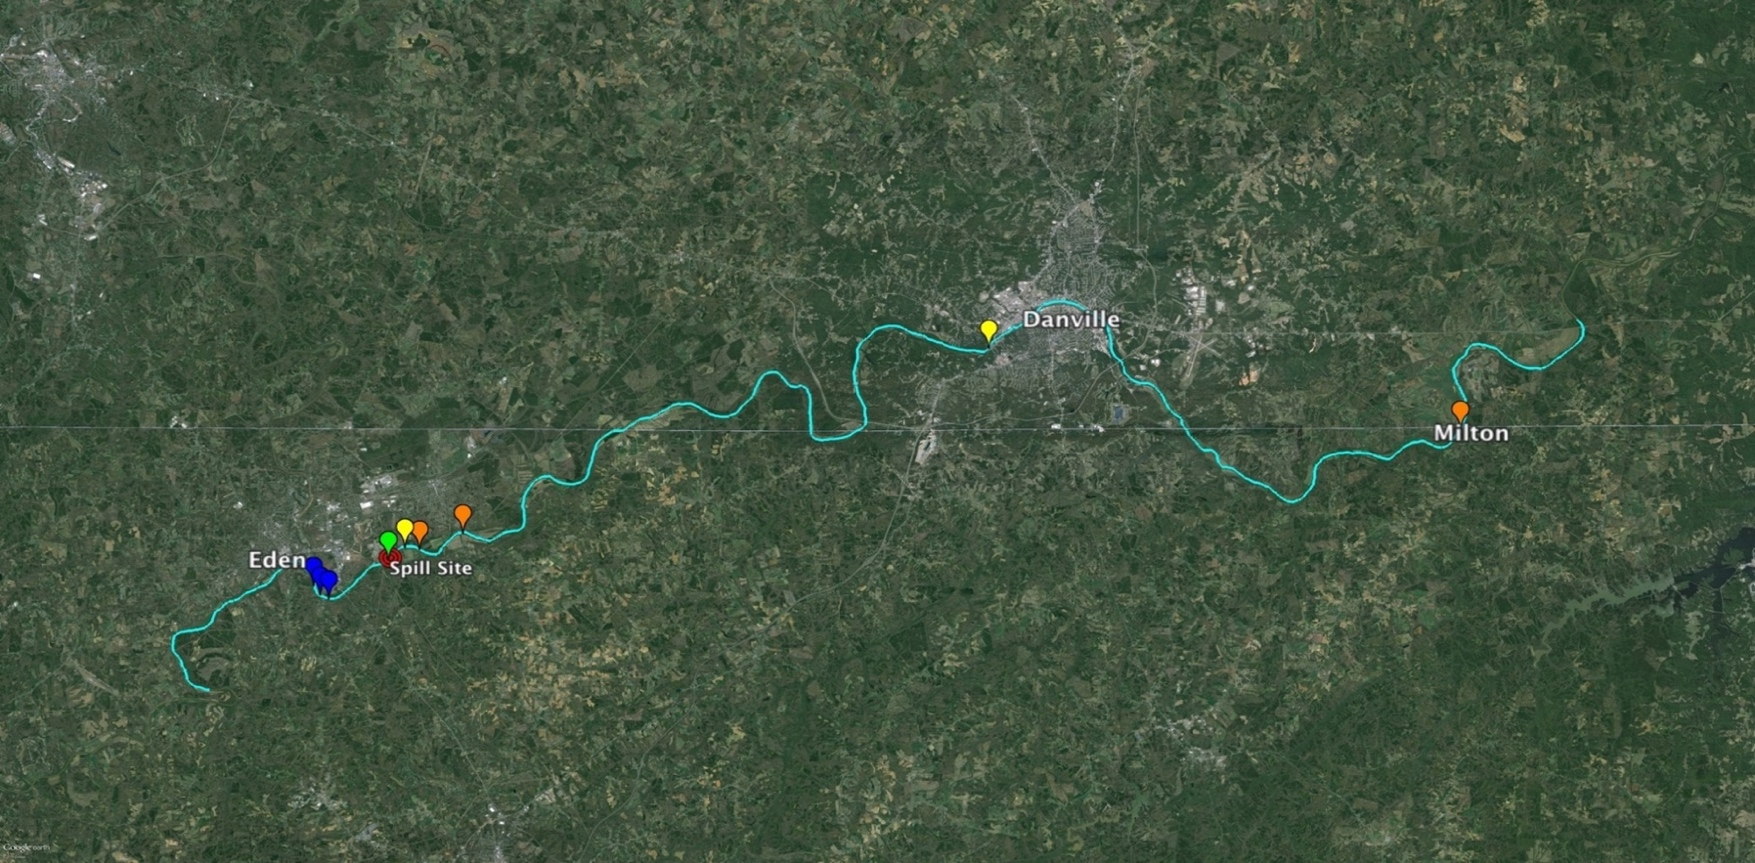
\includegraphics[width=375pt]{figure/map}
  \singlespace \caption[Google Earth Image of Dan River and Sampling Locations.]{Google Earth Image of Dan River and Sampling Locations. Markers indicate sampling sites: Blue, upstream of spill site; Green, leaching site; Yellow, downstream dredged locations; Orange, downstream not dredged.}\label{fig:map}
\end{figure}

Each site was accessed by boat, where sediment from the riverbank and channel was collected. Riverbank sediment cores were collected in triplicate using a piston-style coring device. Channel samples were collected using a small dredge. Sediment cores were sectioned by depth and individual segments homogenized according to one of three sampling schemes to reduce the total number of samples to be assayed (Table \ref{tab:scheme}). 0.25 \(\mathrm{cm^3}\) samples were preserved in CTAB (cetyltrimethylammonium bromide) for DNA extraction. Channel sediment was homogenized then 0.25 \(\mathrm{cm^3}\) was preserved in CTAB.
This field study was constrained by access with few boat ramps, and two dams. River gauge height also provided a logistical obstacle for repeated field sampling. Additionally, the leaching site was accessed after permission from Duke Energy using their onsite boat ramp.
\begin{table}[htbp]

\caption{\label{tab:sites}Sampling Locations.}
\centering
\begin{tabular}{>{\centering\arraybackslash}p{1.5cm}>{\centering\arraybackslash}p{1.5cm}c>{\centering\arraybackslash}p{1.5cm}>{\centering\arraybackslash}p{1.5cm}>{\centering\arraybackslash}p{1.5cm}}
\toprule
Site ID & Distance from Spill (km) & Longitude and Latitude & Sampling Scheme & Shore Samples (n) & Channel Samples (n)\\
\midrule
U-03 & 3.6 & N 36 28.605, W 079 45.018 & B & 6 & 1\\
U-02 & 2.7 & N 36 28.261, W 079 44.598 & C & 4 & 1\\
U-01 & 1.6 & N 36 28.574, W 079 43.989 & A & 2 & 1\\
L-01 & 0.0 & N 36 29.188, W 079 43.025 & B & 6 & 0\\
D-01 & 0.3 & N 36 29.471, W 079 42.722 & B & 6 & 1\\
D-02 & 1.0 & N 36 29.895, W 079 40.836 & C & 4 & 1\\
D-03 & 4.3 & N 36 34.716, W 079 29.596 & C & 5 & 1\\
D-04 & 36.6 & N 36 34.514, W 079 27.024 & B & 6 & 1\\
D-05 & 38.0 & N 36 34.448, W 079 26.211 & A & 3 & 1\\
D-06 & 64.7 & N 36 32.279, W 079 13.038 & A & 2 & 1\\
\bottomrule
\end{tabular}
\end{table}
\begin{table}[htbp]

\caption{\label{tab:scheme}Sediment Sampling Schemes.}
\centering
\begin{tabular}{c>{\centering\arraybackslash}p{10cm}c}
\toprule
Scheme & Description & Total (n)\\
\midrule
A & Triplicate cores segmented at 8 cm and 16 cm, segments pooled & 2\\
B & Triplicate cores segmented at 8 cm and 16 cm, each core sampled & 6\\
C & Triplicate sediment cores pooled at 0-4 cm, 4-8 cm, 8-12 cm, 12-16 cm & 4\\
\bottomrule
\end{tabular}
\end{table}
\hypertarget{dna-extraction-and-qpcr}{%
\subsection{DNA Extraction and qPCR}\label{dna-extraction-and-qpcr}}

A CTAB extraction of DNA was performed using standard protocol for each sample (Stewart and Via, 1993). The DNA extracted was quantified and subsequently diluted to a standard concentration of 5 ng/L in TE (Tris-EDTA) buffer pH 8.0 and stored at 4ºC. Extracted DNA quantity and purity were determined from 2 µL subsamples of each extraction using Thermo Scientific Nanodrop Spectrophotometer based on the 260/280 nm wavelength ratio.

An Applied Biosystems StepOne real-time PCR System was utilized to detect, amplify, and quantify target DNA and representative taxa to meet the objective. Primers were chosen from literature targeting a general metabolic category. These include generic primers to the \emph{hgcA} gene, a sulfate reducing gene, \emph{dsr}, and the 16S rDNA of iron reducing bacteria. (Geets \emph{et al.} (2006);Schaefer \emph{et al.} (2014);Wagner \emph{et al.} (1998);Daly \emph{et al.} (2000), Table \ref{tab:primers}). Each reaction contained the following: 10 µL of Power Sybr® Green PCR master mix, 1 µL of forward primer, 1 µL of reverse primer, 8 µL of sterile deionized water, and 1 µL of extracted DNA. Three negative control reactions, samples repeated in triplicate, and positive standard controls serially diluted in triplicate, were ran in each 48 well plate. Extracted DNA from a pure culture of \emph{Desulfovibrio africanus} (ATCC 19997), an isolate known to contain the \emph{hgcA} gene was used as a standard for the \emph{hgcA} and SRB targets. Genomic DNA extracted from \emph{Geobacter metallireducens} (ATCC 53774) served as the positive control and standard for FeRB primers. The real-time qPCR run method consisted of a holding stage for 5 minutes at 95ºC, followed by 40 cycles of 15 seconds at 95ºC, 1 minute at 57ºC, one minute at 72ºC, and a 15-second data collection at 80ºC, followed by a melt curve analysis beginning at 95ºC, dropping to 60ºC and increasing at 0.3ºC every second until it reaches 95ºC. The relative abundance of targets was computed by the StepOne software using the standard curve. The melt curve was examined to ensure amplicon specificity.

The target abundance was normalized to the volume of extracted sediment as well as to organic matter. The amount of organic matter present in each sample was determined by ash free dry mass (AFDM). Each sample was dried at 60ºC for 48 hours, then combusted in a muffle furnace at 500ºC for 2 hours. Samples were weighed before and after combustion to calculate the AFDM.
\begin{table}[htbp]

\caption{\label{tab:primers}Primers Used in this Study.}
\centering
\begin{tabular}{llll}
\toprule
Target & Primer Name & Primer Sequence 5’-3’ & Reference\\
\midrule
\em{hgcA} & hgcA4R & CGCATYTCCTTYTYBACNCC & Liu \emph{et al.,} 2014\\
 & hgcA4F & GGNRTYAAYRTCTGGTGYGC & \\
FeRB & Geo-R & TACCCGCTACACCTAGT & Medihala \emph{et al.,} 2012\\
 & Geo-F & AGGAAGCAACGGCTAACTCC & \\
SRB & DSV230R & GRGYCYGCGTYYCATTAGC & Daly \emph{et al.,} 2000\\
 & DSV838F & SYCCGRCAYCTAGYRTYCATC & \\
\bottomrule
\end{tabular}
\end{table}
\hypertarget{statistical-analysis}{%
\subsection{Statistical Analysis}\label{statistical-analysis}}

Statistical analyses included nonparametric tests for significance to determine the overall effect of sampling location on the abundance of target per sample. To determine whether abundance of the targets vary in the shore sediment based on the distance from the spill site, the data was first tested for normality with the Shapiro-Wilk test of normality. The data did not follow a Gaussian distribution, therefore, the data were transformed (LN(x +1)), but still failed the test for normality. Samples were binned according to location irrespective of depth due to limited replication of depths, and evaluated with nonparametric tests. For each target, a Kruskall-Wallis test was performed to assess whether a difference in target abundance exists between sites. Where a significant difference was observed, a Wilcoxon Rank Sum test was performed post hoc to determine differences between the location directly downstream of the spill site and all other locations independently. Target abundance of the leaching site was also compared to all other sites. These tests were then repeated with the data normalized to the mass of sediment and to the amount of organic matter present in each sample.

Due to the lack of replication of river channel samples, the samples collected from the river channel bottom were binned into upstream and downstream groups. A Wilcoxon Rank Sum test was used to determine significance. All analyses were conducted using R (R Core Team, 2019).

\hypertarget{results}{%
\section{Results}\label{results}}

\hypertarget{shore-sediment-samples}{%
\subsection{Shore Sediment Samples}\label{shore-sediment-samples}}

The Kruskall-Wallis test revealed a significant difference between the abundance of amplified DNA and sampling locations for each of the three qPCR targets assessed (Kruskall-Wallis p-value \textless0.05). Each of the targets amplified from the D-01 sampling site, the first sampling site downstream (0.3 km) from the spill site, was detected at a higher abundance compared to at least one of the sites downstream and upstream (Figures \ref{fig:hgcaomp} - \ref{fig:srbomp}, Table \ref{tab:compare}). However, D-01 was not the location with the highest overall abundance of these targets. The sampling location U-03, the farthest upstream location, 3.6 km upstream of the spill, and 0.5 km downstream from the Smith River confluence, showed the highest values for each of the targets tested (Figures \ref{fig:hgcaomp} - \ref{fig:srbomp}, Table \ref{tab:compareU}).
\begin{figure}[htbp]
  \includegraphics[width=400pt]{figure/hgcaomp}
   \caption[\textit{hgcA} Abundance Normalized to Organic Matter at Each Sampling Location.]{\textit{hgcA} Abundance Normalized to Organic Matter at Each Sampling Location. Asterisks signify difference between the reference, D-01 using the Wilcoxon Rank Sum test. * : p <= 0.05, ** : p <= 0.01}\label{fig:hgcaomp}
\end{figure}
\begin{figure}[htbp]
  \includegraphics[width=400pt]{figure/ferbomp}
   \caption[FeRB Abundance Normalized to Organic Matter at Each Sampling Location.]{FeRB Abundance Normalized to Organic Matter at Each Sampling Location. Asterisks signify difference between the reference, D-01 using the Wilcoxon Rank Sum test. * : p <= 0.05, ** : p <= 0.01}\label{fig:ferbomp}
\end{figure}
\begin{figure}[htbp]
  \includegraphics[width=400pt]{figure/srbomp}
   \caption[SRB Abundance Normalized to Organic Matter at Each Sampling Location.]{SRB Abundance Normalized to Organic Matter at Each Sampling Location. Asterisks signify difference between the reference, D-01 using the Wilcoxon Rank Sum test. * : p <= 0.05, ** : p <= 0.01}\label{fig:srbomp}
\end{figure}
\begin{table}[htbp]

\caption[Comparisons of Each Sampling Location to the Location Directly Downstream of the Spill.]{\label{tab:compare}Comparisons of Each Sampling Location to the Location Directly Downstream of the Spill. Wilcoxon Rank Sum Test, ns: not significant, * : p <= 0.05, ** : p <= 0.01}
\centering
\begin{tabular}{llll}
\toprule
Location & \textit{hgcA} & FeRB & SRB\\
\midrule
U-03 & ns & ** & ns\\
U-02 & ** & ns & *\\
U-01 & ns & ns & ns\\
L-01 & ns & ns & ns\\
D-02 & ** & ** & **\\
D-03 & ns & * & *\\
D-04 & ns & ns & ns\\
D-05 & * & * & *\\
D-06 & ns & ns & ns\\
\bottomrule
\end{tabular}
\end{table}
\begin{table}[htbp]

\caption[Comparisons of Each Sampling Location to the Furthest Upstream Location.]{\label{tab:compareU}Comparisons of Each Sampling Location to the Furthest Upstream Location. Wilcoxon Rank Sum Test, ns: not significant, * : p <= 0.05, ** : p <= 0.01}
\centering
\begin{tabular}{llll}
\toprule
Location & \textit{hgcA} & FeRB & SRB\\
\midrule
U-03 & ns & ** & ns\\
U-02 & ** & ns & *\\
U-01 & ns & ns & ns\\
L-01 & ns & ns & ns\\
D-02 & ** & ** & **\\
D-03 & ns & * & *\\
D-04 & ns & ns & ns\\
D-05 & * & * & *\\
D-06 & ns & ns & ns\\
\bottomrule
\end{tabular}
\end{table}

Additionally, the leaching site, L-01 is not significantly different from the D-01 location. When comparing the leaching site to all others, targets abundance is slightly higher than most of the other sampling locations. This pattern is similar to the D-01 comparisons, but overall, less pairs are significantly different (Table \ref{tab:compareL}). The same pattern was observed between the data normalized to the mass of sediment in each sample as well as the amount of organic matter present.
\begin{table}[htbp]

\caption[Comparisons of Each Sampling Location to the Leaching Site Location.]{Comparisons of Each Sampling Location to the Leaching Site Location. Wilcoxon Rank Sum Test, ns: not significant, * : p <= 0.05, ** : p <= 0.01}{\label{tab:compareL}
\centering
\begin{tabular}{llll}
\toprule
Location & \textit{hgcA} & FeRB & SRB\\
\midrule
U-03 & ns & ** & ns\\
U-02 & ** & ns & *\\
U-01 & ns & ns & ns\\
L-01 & ns & ns & ns\\
D-02 & ** & ** & **\\
D-03 & ns & * & *\\
D-04 & ns & ns & ns\\
D-05 & * & * & *\\
D-06 & ns & ns & ns\\
\bottomrule
\end{tabular}
\end{table}

Within this study, replication of core depth was limited, therefore, the interaction between the depth of samples was not evaluated. However, a scatterplot of the data did not show any clear patterns indicating a depth interaction, but the effect is inconclusive (Figure \ref{fig:depth}).

\begin{figure}[htbp]
\includegraphics[width=400pt]{figure/depth}
   \caption[Target DNA Concentration at Each Depth]{Target DNA Concentration at Each Depth.}
   \label{fig:depth}
   \end{figure}
\hypertarget{river-channel-samples}{%
\subsection{River Channel Samples}\label{river-channel-samples}}

The samples collected in the river channel were limited by one sample at each site. To assess significance, samples were binned according to upstream and downstream. For each of the targets tested, there is no significant difference between the groups (Figure \ref{fig:channel}).

\begin{figure}[htbp]
  \includegraphics[width=400pt]{figure/channel}
  \caption[River Channel Abundance at Sampling Sites Upstream and Downstream Normalized to Organic Matter.]{River Channel Abundance at Sampling Sites Upstream and Downstream Normalized to Organic Matter.}\label{fig:channel}
\end{figure}
\hypertarget{discussion}{%
\section{Discussion}\label{discussion}}
\addtocontents{toc}{\vspace{\normalbaselineskip}}

The abundance of targets detected at the sampling location 0.3 km downstream of the spill site, D-01, is higher than some locations upstream and downstream. However, the highest abundance of these three targets was found at the furthest upstream site of all locations. Notably, the leaching site, L-01, and D-01 were not significantly different, and also exhibited higher target signal over some locations. This may signify that there is an impact from leaching of coal ash constituents. All primers tested exhibited similar patterns of significance and abundance per location. We experienced technical difficulties when assaying additional primer sets (Christensen \emph{et al.}, 2016)
leading to a smaller suite of targets to determine overall microbial community response to the coal ash spill.

The results from this microbial study are inconclusive. Our findings indicate that a significant difference exists between some of the sampling locations and the location directly downstream of the spill site, but the highest signal for each target was found at the furthest location upstream from the spill. Hg contamination within the sediment may still be possible, and our methods of sampling sediment may not have been robust to the variable and ``hotspot'' nature of the coal ash deposition and dispersal into the river sediments. It is plausible that the coal ash is buried in the sediment or has been transported further downstream than our furthest downstream location 1.5 years after the spill event.

\hypertarget{metal}{%
\chapter{IDENTIFICATION AND CHARACTERIZATION OF HEAVY METAL TOLERANCE OF BACTERIA ISOLATED FROM COAL ASH}\label{metal}}

\hypertarget{introduction-1}{%
\section{Introduction}\label{introduction-1}}

Coal ash is a waste product generated from coal-fired power plants. These power plants are located near water sources to meet water demands during the electricity generation process. The ash and other waste products are discharged as a slurry into a settling pond, after the combustion process (Connors, 2015). To prevent overflow the pond is maintained by pumping surface water into the nearby waters, usually a river. In North Carolina, 14 such coal ash ponds are maintained by Duke Energy. Unlined and uncapped coal ash waste ponds therefore have the potential for leaching contaminants into the groundwater or spilling into nearby waterways possibly polluting drinking water and/or disrupting aquatic ecological communities (Otter \emph{et al.}, 2012; Ruhl \emph{et al.}, 2009).

On February 2, 2014, a coal ash pond located at the retired Dan River Steam Station near Eden, NC expelled approximately 39,000 tons of coal ash slurry into the Dan River of North Carolina due to an underground pipe collapse (NC DEQ, 2014). The ash was dispersed along the river bottom between the spill site and the Kerr Reservoir, approximately 120 km downstream (Hesterberg \emph{et al.}, 2014). Dredging operations conducted by Duke Energy at Town Creek and an area upstream from the Schoolfield Dam in Danville, VA, removed approximately 2,500 tons of coal ash-laden sediment, but the remainder was deposited in the river bottom (Lemly, 2015).

Physical and chemical properties of coal ash are determined by the geographic location where the raw coal was mined, the type of boiler, and the operating conditions of the power plant (Jayaranjan \emph{et al.}, 2014). All natural elements can be found in coal ash including trace elements such as arsenic, cadmium, chromium, mercury, lead, selenium, and zinc (Greely Jr. \emph{et al.}, 2014; Jayaranjan \emph{et al.}, 2014). Coal ash is wholly comprised of multiple waste products with differing chemical properties including fly ash, bottom ash, and byproducts of pollution mitigation processes, such as scrubber systems. Fly ash is composed mainly of oxides such as, \(\mathrm{SiO_2}\), \(\mathrm{Al_2O}\), \(\mathrm{Fe_2O}\). Bottom ash consists of silicate, carbonate, aluminate, ferrous materials and high concentrations of several heavy metals and metalloids (Kisku \emph{et al.}, 2018).

Heavy metals are characterized by a density greater than 5 g/\(\mathrm{cm^3}\), mostly transition elements, and play an important role as trace elements in biochemical reactions. These heavy metals, due to an incompletely filled d orbital, allow the cations to form complex compounds with the potential to be redox reactive. Heavy metal ions form unspecific complex compounds in living cells, leading to toxic effects. For example, \(\mathrm{Hg^{2+}}\), \(\mathrm{Cd^{2+}}\), and \(\mathrm{Ag^{+}}\) form strong toxic complexes that are not conducive to any physiological function. Trace metals such as \(\mathrm{Zn^{2+}}\), \(\mathrm{Ni^{2+}}\), and \(\mathrm{Cu^{2+}}\) are required for some biological functions but they are toxic at high concentrations Hesterberg \emph{et al.} (2014). Therefore, the intracellular concentration of heavy metals must be controlled, and organisms have adapted heavy metal resistance strategies (Binkley and Simpson, 2003; Poulain and Barkay, 2013).

Through the process of coal combustion, the coal ash is rendered sterile. Therefore, inoculation of coal ash in waste ponds occurs by natural processes including atmospheric deposition through rainfall and windblown particulates. Opportunistic microorganisms may be adapted, or may be able to adapt, to the high concentration of heavy metals through resistance or metal detoxification. Perturbations such as coal ash spills result in altered environments in receiving waters, which microbes may adapt to and subsequently mobilize coal ash constituents into food webs. Knowledge of the microbial community structure and distribution is important to estimate the extent of biological mobility of these pollutants. Further, organisms which exhibit metal tolerance may warrant further investigation into their potential for bioremediation (Keshri \emph{et al.}, 2014; Naik and Dubey, 2013; Pepi \emph{et al.}, 2011; Raja and Omine, 2012).

The objective of this study was to determine if a microbial community is viable and present in coal ash ponds, and if present, identify the taxa and assess the metal tolerance of isolated organisms. Previous studies have analyzed the microbial community of soils amended with coal ash (Klubek \emph{et al.}, 1992). No studies to date have determined the microbial community of coal ash alone. In a preliminary PCR analysis, a small amount of DNA was present in a coal ash sample from the Dan River Steam Station coal ash pond, but we were not able to amplify SSU rDNA from bacteria with universal prokaryotic primers, possibly due to contaminants present in the sample or low concentrations of bacterial DNA. Therefore, in this study, we increased the abundance of microbes and their DNA by culturing and isolating bacteria from samples of coal ash, to ensure adequate amounts of DNA for analyses.

\hypertarget{objectives-and-hypotheses}{%
\subsection{Objectives and Hypotheses}\label{objectives-and-hypotheses}}

\textbf{Objective 1: To identify isolated bacteria using qPCR amplification and rDNA sequencing. I seek to identify these taxa using qPCR amplification and rDNA sequencing to compare to the GenBank database.}

\emph{I hypothesize novel organisms may be discovered which may have unique metal tolerance capabilities that may be useful for bioremediation.}

\textbf{Objective 2: To determine the metal tolerance of bacteria isolated from coal ash collected from the Dan River impoundment site.}

\emph{I hypothesize that microbial growth of bacterial isolates from pure coal ash collected at the Dan River Steam Station impoundment pond will be more tolerant to heavy metals than organisms isolated from a reference site (soil collected from Peabody Park on UNCG campus).}

\hypertarget{methods-1}{%
\section{Methods}\label{methods-1}}

\hypertarget{pure-culture-isolation-from-coal-ash}{%
\subsection{Pure Cculture Isolation from Coal Ash}\label{pure-culture-isolation-from-coal-ash}}

Samples of coal ash provided by our collaborator, Brian Williams of the Dan River Basin Association, were taken directly from a coal ash retention pond at the retired Dan River Steam Station near Eden, NC. To culture isolated organisms, aliquots (0.5 g) of coal ash from the pond were added to six 50 mL conical tubes. 40 mL of filter sterilized (0.22 µm pore) Dan River water was added to three tubes and filter sterilized Dan River water supplemented with 10\% nutrient broth to the other three tubes. Additionally, filter sterilized Dan River water alone was evaluated in triplicate to serve as a sterility control. Tubes were incubated at ambient room temperature for 48 hours without agitation. 1 mL aliquots were then transferred from each culture and spread on 50\% nutrient agar plates for isolation. Morphologically unique colonies identified on spread plates were isolated and pure cultures maintained on 50\% nutrient agar slants for heavy metal tolerance experimentation. Sediment samples collected from Peabody Park, UNCG campus, used as a comparison, were isolated using the same protocol as described.

\hypertarget{heavy-metal-tolerance-characterization}{%
\subsection{Heavy Metal Tolerance Characterization}\label{heavy-metal-tolerance-characterization}}

Optical density (OD) at 580 nm, of liquid broth culture was assessed as a proxy for growth of organisms, since growth is related to the increase in turbidity of a bacterial culture. Metals tested include, arsenic, cadmium, chromium, mercury, lead, selenium and zinc. Stock concentrations of \(\mathrm{Na_2HAsO_4}\), \(\mathrm{CdCl_2}\), \(\mathrm{CrCl_3}\), \(\mathrm{HgCl_2}\), \(\mathrm{PbCl_2}\), \(\mathrm{Na_2SeO_3}\), and \(\mathrm{ZnCl_2}\) were serially diluted to span several orders of magnitude greater and less than natural environmental concentrations reported in the literature for each metal, resulting in five concentration levels per metal (Table \ref{tab:metals}).
\begin{table}[htbp]
\caption[Final Concentrations of Metal in Fermentation Broth.]{Final Concentrations of Metal in Fermentation Broth (µg/L).}\label{tab:metals}
\centering
\begin{tabular}{cccccccc}
\toprule
Factor & As & Cd & Cr & Hg & Pb & Se & Zn\\
\midrule
1 & 0.001 & 0.001 & 0.01 & 0.001 & 0.01 & 1 & 0.1\\
2 & 0.010 & 0.010 & 0.10 & 0.010 & 0.10 & 10 & 1.0\\
3 & 0.100 & 0.100 & 1.00 & 0.100 & 1.00 & 100 & 10.0\\
4 & 1.000 & 1.000 & 10.00 & 1.000 & 10.00 & 1000 & 100.0\\
5 & 10.000 & 10.000 & 100.00 & 10.000 & 100.00 & 10000 & 1000.0\\
\bottomrule
\end{tabular}
\end{table}

Metal stocks were prepared by dissolving each metal salt in sterile reverse osmosis deionized (RO/DI) water and subsequently diluted. To ensure a viable culture inoculum, sufficient volume of cells, and standardization for experimentation, each unique isolate was incubated in a 50\% nutrient broth culture in a shaking water bath at 25ºC overnight until an optical density of at least 0.7 at 580 nm was observed. For each metal-isolate experiment, 100 µL of 0.7 OD\textasciitilde580 nm\textasciitilde{} inoculum was added to 2.4 mL of 50\% nutrient broth amended with 100 µL each concentration of metal in triplicate. For the control, 100 µL of RO/DI water was substituted for the metal spike in triplicate. Growth patterns were measured by absorbance at 580 nm, and recorded at ten time points, approximately 0, 1, 2, 4, 8, 16, 24, 30, 36, and 48 hours post inoculation.

\hypertarget{isolate-identification-and-phylogenetic-analysis}{%
\subsection{Isolate Identification and Phylogenetic Analysis}\label{isolate-identification-and-phylogenetic-analysis}}

Isolates were grown in 50\% nutrient broth then pelleted by centrifugation. The pellet was resuspended in CTAB buffer. DNA was extracted and purified using the CTAB method (Stewart and Via, 1993), then amplified with universal 16S primers (Bruce \emph{et al.}, 1992; Edwards \emph{et al.}, 1989). PCR products were then purified and commercially sequenced. Sequence chromatogram data was evaluated and edited manually to optimize the sequence. The FASTA files of sequences were imported into Molecular Evolutionary Genetics Analysis version 7.0 (MEGA7) (Kumar \emph{et al.}, 2016). Sequences were aligned using MUSCLE and manual adjustments (Edgar, 2004). The resulting aligned sequences were then subjected to phylogenetic tree analysis using MEGA7. The maximum likelihood tree was computed using MEGA7 using the Jukes-Cantor model (Jukes and Cantor, 1969). The bootstrap consensus tree was inferred from 1000 replicates. Initial trees with a greater log likelihood value were calculated by applying Neighbor-Join and BioNJ algorithms to a matrix of pairwise distances estimated using the Maximum Composite Likelihood approach. To identify the genus of each isolate, the sequences were compared to the NCBI GenBank database with BLASTn (Nucleotide Basic Local Alignment Search Tool). Genus calls were made with similarities greater than 97\% (Clark \emph{et al.}, 2016).

\hypertarget{statistical-analyses}{%
\subsection{Statistical Analyses}\label{statistical-analyses}}

To characterize the heavy metal tolerance of isolates in liquid broth culture, the carrying capacity and growth rate of each isolate-metal experiment was modeled with a Gompertz sigmoidal function (Zwietering \emph{et al.}, 1990). Significant differences of growth rate and carrying capacity within each experiment were determined using the Kruskall-Wallis one-way analysis of variance test (p-value \textless{} 0.05). Experiments were excluded from analysis where no growth was observed in the control. Isolates were deemed metal tolerant at the concentrations tested if no significant difference between carrying capacity or growth rate was observed between concentrations.

\hypertarget{results-1}{%
\section{Results}\label{results-1}}

\hypertarget{phylogenetic-analysis}{%
\subsection{Phylogenetic Analysis}\label{phylogenetic-analysis}}

A total of 31 microorganisms were isolated from the coal ash sample and sequenced, five were isolated from Peabody Park soil for comparison to coal ash samples as ``control'' samples. The soil samples are assumed to be free of coal ash, but these soils were probably affected by farming practices in the past, which may have included introduction of heavy metals to the soil. Sequences were aligned and a phylogenetic tree was constructed (Figure \ref{fig:tree}). Sequences were predominantly identified as \emph{Bacillus} or \emph{Arthrobacter} spp. One isolate, DR 76, was not identified in GenBank with the BLASTn search. Of the 5 isolates that were cultured from soil, three are identified as \emph{Bacillus} sp., one \emph{Duganella}, and one \emph{Pseudomonas}. \emph{Duganella} and \emph{Pseudomonas} were unique to the soil samples.
\begin{figure}[htbp]
  \centering
  \includegraphics[width=375pt]{figure/tree6}
  \caption[Phylogenetic Analysis of Isolates Cultured from Coal Ash Amended Media.]{Phylogenetic Analysis of Isolates Cultured from Coal Ash Amended Media. Identification of Coal ash-free isolates are prepended with S1-S5, all others are coal ash samples.}\label{fig:tree}
\end{figure}

\hypertarget{metal-tolerance-assays}{%
\subsection{Metal Tolerance Assays}\label{metal-tolerance-assays}}

We tested metal tolerance of 16 isolates. When exposed to a heavy metal, isolates generally grew well (Figures \ref{fig:si4} - \ref{fig:dr52}). The isolates were challenged against seven metals, resulting in a total of 94 trials. 17 trials were excluded due to lack of growth e.g.~Figure \ref{fig:dr52} Se. There was little difference between coal ash isolates and a ``control'', SI 4 (Figure \ref{fig:si4}). In one of the ``control'' isolates, SI 2, growth was not observed and was excluded. The soil isolate SI 4, was tolerant to all metals at the concentrations tested except for cadmium and zinc (Tables \ref{tab:kpvalue} and \ref{tab:muvalue}, Figure \ref{fig:si4}).

When evaluating carrying capacity, 70 trials were not different from the control, Kruskall-Wallis test p-value \textgreater0.05 (Table \ref{tab:kpvalue}). Evaluation of maximal growth rate produced 71 isolate-metal trials that were not significantly different (Table \ref{tab:muvalue}). 64\% of the isolates tested were susceptible to Cd and 72\% are susceptible to Se. The other metals tested (As, Cr, Hg, Pb, and Zn) resulted in much less susceptibility, ranging from 1-3 susceptible isolates.
\begin{figure}
   \centering
   \includegraphics[width=400pt]{figure/si4plot}
   \caption[Growth of Soil Isolate SI4.]{Growth of Soil Isolate SI4. Lines connect means of three replicates, colors represent concentration levels (Table 3.1). Carrying capacity is not significantly different between metal concentrations. Growth rates are different in Cd and Zn experiments (Kruskall-Wallis test p-value < 0.05)}\label{fig:si4}
\end{figure}
\begin{figure}
    \centering
    \includegraphics[width=400pt]{figure/dr13plot}
    \caption[Growth of Isolate DR13.]{Growth of Isolate DR13. Lines connect means of three replicates, colors represent concentration levels (Table 3.1). Carrying capacity is significantly different between metal concentrations of Cd and Zn.  Growth rates are different with As and Zn (Kruskall-Wallis test p-value < 0.05)}\label{fig:dr13}
\end{figure}
\begin{figure}
  
  \centering
    \includegraphics[width=400pt]{figure/dr32plot}
    \caption[Growth of Isolate DR3.2.]{Growth of Isolate DR3.2. Lines connect means of three replicates, colors represent concentration levels (Table 3.1). Carrying capacity is significantly different between metal concentrations of Cd and Se. No difference is observed when testing maximal growth rates (Kruskall-Wallis test p-value < 0.05)}\label{fig:dr32}
\end{figure}
\begin{figure}
  
  \centering
    \includegraphics[width=400pt]{figure/dr52plot}
    \caption[Growth of Isolate DR52.]{Growth of Isolate DR52. Lines connect means of three replicates, colors represent concentration levels (Table 3.1). Se was excluded from analysis. Carrying capacity is significantly different between metal concentrations of Cd. Growth rates are different with As, Cd, and Hg. (Kruskall-Wallis test p-value < 0.05) }\label{fig:dr52}
\end{figure}
\begin{table}[htbp]

\caption[P-values of Kruskall-Wallis Test of Carrying Capacity.]{\label{tab:kpvalue}P-values of Kruskall-Wallis Test of Carrying Capacity. Bold typeface signifies p-value <0.05. NA: Not Analyzed}
\centering
\resizebox{\linewidth}{!}{
\begin{tabular}{lllllllll}
\toprule
\multicolumn{1}{c}{Genus} & \multicolumn{1}{c}{Isolate} & \multicolumn{1}{c}{As} & \multicolumn{1}{c}{Cd} & \multicolumn{1}{c}{Cr} & \multicolumn{1}{c}{Hg} & \multicolumn{1}{c}{Pb} & \multicolumn{1}{c}{Se} & \multicolumn{1}{c}{Zn}\\
\midrule
\rowcolor{gray!6}  Not Sequenced & DR13 & 0.138 & \textbf{0.046} & 0.148 & 0.086 & 0.281 & 0.083 & \textbf{0.025}\\
\em{Arthrobacter} & DR24 & 0.141 & \textbf{0.025} & 0.554 & 0.504 & 0.163 & NA & \textbf{0.022}\\
\rowcolor{gray!6}  \em{Sinomonas} & DR26 & 0.482 & \textbf{0.02} & 0.612 & 0.547 & 0.134 & \textbf{0.011} & 0.067\\
\em{Arthrobacter} & DR3.2 & 0.367 & \textbf{0.027} & 0.637 & 0.091 & 0.669 & \textbf{0.011} & 0.344\\
\rowcolor{gray!6}  \em{Arthrobacter} & DR5 & 0.171 & 0.203 & 0.961 & 0.494 & 0.075 & 0.074 & 0.16\\
\em{Bacillus} & DR52 & 0.364 & \textbf{0.009} & 0.691 & 0.425 & 0.066 & NA & 0.081\\
\rowcolor{gray!6}  \em{Arthrobacter} & DR60 & \textbf{0.038} & \textbf{0.04} & 0.097 & 0.135 & 0.074 & NA & 0.164\\
Unknown Genus & DR76 & 0.125 & 0.336 & 0.517 & NA & 0.18 & \textbf{0.014} & \textbf{0.02}\\
\rowcolor{gray!6}  \em{Bacillus} & DRp51 & 0.116 & \textbf{0.014} & 0.54 & 0.713 & 0.787 & \textbf{0.008} & 0.193\\
\em{Lynsinibacillus} & DRp72 & 0.173 & \textbf{0.018} & 0.096 & 0.057 & 0.43 & NA & 0.104\\
\rowcolor{gray!6}  \em{Pelemonas} & DRp74 & 0.385 & 0.105 & \textbf{0.015} & \textbf{0.016} & 0.131 & \textbf{0.032} & 0.669\\
Not Sequenced & NO14 & 0.243 & \textbf{0.031} & 0.297 & 0.97 & 0.822 & \textbf{0.03} & 0.741\\
\rowcolor{gray!6}  Not Sequenced & NO17 & 0.051 & 0.067 & 0.22 & 0.329 & \textbf{0.035} & 0.054 & 0.063\\
Not Sequenced & NO22 & NA & NA & NA & NA & NA & \textbf{0.014} & NA\\
\rowcolor{gray!6}  \em{Bacillus} & SI2 & NA & NA & NA & NA & NA & \textbf{0.01} & NA\\
\em{Dunganella} & SI4 & 0.361 & 0.076 & 0.255 & 0.09 & 0.983 & NA & 0.051\\
\bottomrule
\end{tabular}}
\end{table}
\begin{table}[!h]

\caption[P-values of Kruskall-Wallis Test of Maximal Growth Rate.]{\label{tab:muvalue}P-values of Kruskall-Wallis Test of Maximal Growth Rate. Bold typeface signifies p-value <0.05. NA: Not Analyzed}
\centering
\resizebox{\linewidth}{!}{
\begin{tabular}{lllllllll}
\toprule
\multicolumn{1}{c}{Genus} & \multicolumn{1}{c}{Isolate} & \multicolumn{1}{c}{As} & \multicolumn{1}{c}{Cd} & \multicolumn{1}{c}{Cr} & \multicolumn{1}{c}{Hg} & \multicolumn{1}{c}{Pb} & \multicolumn{1}{c}{Se} & \multicolumn{1}{c}{Zn}\\
\midrule
\rowcolor{gray!6}  Not Sequenced & DR13 & \textbf{0.042} & 0.177 & 0.445 & 0.825 & 0.251 & 0.114 & \textbf{0.021}\\
\em{Arthrobacter} & DR24 & 0.284 & \textbf{0.026} & 0.073 & 0.183 & 0.637 & NA & \textbf{0.02}\\
\rowcolor{gray!6}  \em{Sinomonas} & DR26 & 0.306 & 0.128 & 0.149 & 0.383 & 0.114 & \textbf{0.009} & 0.334\\
\em{Arthrobacter} & DR3.2 & 0.206 & 0.068 & 0.171 & 0.074 & 0.213 & 0.055 & 0.083\\
\rowcolor{gray!6}  \em{Arthrobacter} & DR5 & 0.419 & \textbf{0.036} & 0.192 & 0.637 & 0.56 & \textbf{0.012} & 0.511\\
\em{Bacillus} & DR52 & \textbf{0.028} & \textbf{0.007} & 0.889 & \textbf{0.041} & 0.063 & NA & 0.078\\
\rowcolor{gray!6}  \em{Arthrobacter} & DR60 & \textbf{0.028} & 0.071 & 0.054 & 0.082 & 0.141 & NA & \textbf{0.03}\\
Unknown Genus & DR76 & 0.218 & 0.451 & 0.534 & NA & 0.399 & \textbf{0.039} & \textbf{0.028}\\
\rowcolor{gray!6}  \em{Bacillus} & DRp51 & 0.154 & 0.138 & \textbf{0.025} & 0.439 & 0.975 & 0.136 & 0.279\\
\em{Lynsinibacillus} & DRp72 & 0.263 & \textbf{0.035} & 0.255 & 0.158 & 0.385 & NA & 0.173\\
\rowcolor{gray!6}  \em{Pelemonas} & DRp74 & 0.669 & 0.261 & \textbf{0.048} & \textbf{0.021} & 0.056 & 0.141 & 0.488\\
Not Sequenced & NO14 & 0.324 & 0.086 & 0.713 & 0.9 & 0.801 & \textbf{0.014} & 0.648\\
\rowcolor{gray!6}  Not Sequenced & NO17 & 0.174 & 0.107 & 0.68 & 0.825 & 0.112 & \textbf{0.013} & 0.286\\
Not Sequenced & NO22 & NA & NA & NA & NA & NA & 0.05 & NA\\
\rowcolor{gray!6}  \em{Bacillus} & SI2 & NA & NA & NA & NA & NA & 0.377 & NA\\
\em{Dunganella} & SI4 & 0.117 & \textbf{0.026} & 0.388 & 0.108 & 0.982 & NA & \textbf{0.036}\\
\bottomrule
\end{tabular}}
\end{table}
\hypertarget{discussion-1}{%
\section{Discussion}\label{discussion-1}}
\addtocontents{toc}{\vspace{\normalbaselineskip}}
We isolated cultures of aerobic bacteria from samples of coal ash. The coal ash isolates are predominantly identified as \emph{Arthrobacter} and \emph{Bacillus} spp. \emph{Arthrobacter} spp. are ubiquitous and have been found in common soils as well as extreme environments. These spore-formers are able to survive long periods of time under stressful conditions such as nutrient deficiency, temperature shifts, and toxic chemicals. \emph{Arthrobacter} sp. are metabolically diverse, have been utilized to biodegrade environmental pollutants, and are highly resistant to heavy metals (Mongodin \emph{et al.}, 2006). We isolated \emph{Arthrobacter} from coal ash samples, but did not isolate them from the soil sample. The predominance of \emph{Arthrobacter} sp. from the coal ash may be due to the selective pressure of the coal ash. High concentrations of Cd had an effect on most of the isolates tested. Of the five isolates that were tolerant of Cd, one is \emph{Arthrobacter}, although not all \emph{Arthrobacter} were tolerant of Cd. \emph{Bacillus} spp. are genomically diverse, ubiquitous endospore-formers are highly resistant to stressors (Earl \emph{et al.}, 2008). Three \emph{Bacillus} spp. were subjected to metal tolerance assays. The soil isolate SI2, a \emph{Bacillus} was only tested for Se, and was susceptible. The other \emph{Bacillus} spp. (DR52 and DRp51) exhibited the same metal tolerance characterization; tolerant to all except Cd and Se.

One isolate could not be identified by a BLASTn search of the GenBank database, and may be an interesting organism to for further testing and characterization. Since we only studied organisms which were easily grown and maintained within the lab under room temperature conditions, likely only a small portion of the organisms present were cultivated. More novel organisms may be discoverable using less selective methods.

These data are suggestive of metal tolerance, and this assay was useful as a screen to find interesting isolates for further study, but these data are not conclusive. Due to a small sample size and unbalanced number of coal ash isolates compared to soil isolates, we are unable to determine if the coal ash samples are more or less tolerant to heavy metals than the soil samples.

\hypertarget{conclusions}{%
\chapter{CONCLUSIONS}\label{conclusions}}

The coal ash spill into the Dan River is the third worst spill in United States history. It released thousands of tons of ash and millions of gallons of untreated coal ash slurry into the Dan River. Approximately 1.5 years after the spill, the microbial response to the influx of coal ash into the sediment of the river was assessed using qPCR to probe samples targeting a mercury-methyating gene, and SSU rDNA from SRB and FeRB. Using these methods, relative to other locations, we found elevated abundance of of the three targets assessed, adjacent to the ponds (leaching site) and the location directly downstream of the spill site. These results may indicate the taxa are responding to the coal ash, but we are unable to provide strong evidence using these methods.

In this study we observed similar patterns of abundance of each target along the distance gradient. This indicates a similar response is detected between multiple taxonomic groups. Unexpectedly, the highest abundance among all targets was observed at a site that seems unlikely to have been contaminated with coal ash due to it's distance upstream from the spill site, where the coal ash was carried away downstream. We were unable to test if the target abundance is impacted by the depth of the sample due to inadequate replication, but we suspect any pattern within depth of sample may relate to the amount organic matter present in the sample, which could be highly variable.

Our sampling effort was constrained by multiple circumstances. The field sampling was limited by access to locations, weather, and river gauge height. We were also limited by the number of samples we were able to process. Additionally, the locations along the river available and selected for study may have been inadequate due to the unpredictability and variability of coal ash depositional sites, or ``hotspots''. These ``hotspots'' with a higher concentration of coal ash may stimulate more bacterial growth than other locations and thus provide a more definitive signal. Potentially, new technologies such as utilizing unmanned aerial vehicles to determine the size and scope of coal ash spills and other environmental pollution events, may aid in identifying hotspots and therefore, improve sampling strategies(Messinger and Silman, 2016).

Our results may also have been improved by assaying additional primers including primers designed to capture a broader suite of \emph{hgcA} containing bacteria. Additionally, testing general bacterial primers to serve as a microbial abundance background to better characterize a possible correlation between the targets.

We also characterized the metal tolerance of bacteria cultivated from coal ash. The observed tolerance among isolates is consistent with previous studies (Klubek \emph{et al.}, 1992; Raja and Omine, 2012). We only tested the growth of the isolates, and did not measure the ion concentrations directly to determine the if the metal was unbound and available for uptake. It is possible, the exposure level was lower than nominal concentrations (Hughes and Poole, 1991; Ramamoorthy and Kushner, 1975).

The coal ash isolates and the soil isolates exhibited similar tolerances. This may indicate the bacteria isolated in the lab may be adapted to high levels of these metals where the soil isolates may be adapted to soil subjected to farming activities in the past. The isolates were identified by SSU rDNA sequencing and all were identified by genus, except one. The BLASTn search returned a sequence that has not been fully characterized for identification. Unsurprisingly, the population of culturable bacteria is represented by genera that are usually found in harsh environments.

The results of this study provide some insights to the response of bacteria to coal ash. If another natural disaster or pollution event were to occur, a similar study with improved sampling methods may help characterize the risk of mercury-methylating stimulation and mobilization into the food webs.

\backmatter

\hypertarget{references}{%
\chapter{REFERENCES}\label{references}}

\noindent

\setlength{\parindent}{-0.20in}
\setlength{\leftskip}{0.20in}
\setlength{\parskip}{8pt}

\hypertarget{refs}{}
\leavevmode\hypertarget{ref-americancoalashassociation2012CoalCombustion2012}{}%
American Coal Ash Association (2012). 2012 Coal Combustion Product (CCP) Production and Use Survey Report (ACAA).

\leavevmode\hypertarget{ref-binkleyHeavyMetalsWastewater2003}{}%
Binkley, J., and Simpson, J.A. (2003). Heavy metals in wastewater treatment processes. In Handbook of Water and Wastewater Microbiology, D.D. Mara, and N.J. Horan, eds. (London ; San Diego: Academic Press), pp. 597--610.

\leavevmode\hypertarget{ref-bizilyPhytoremediationMethylmercuryPollution1999}{}%
Bizily, S.P., Rugh, C.L., Summers, A.O., and Meagher, R.B. (1999). Phytoremediation of methylmercury pollution: merB expression in Arabidopsis thaliana confers resistance to organomercurials. PNAS \emph{96}, 6808--6813.

\leavevmode\hypertarget{ref-boydMercuryResistanceOperon2012}{}%
Boyd, E., and Barkay, T. (2012). The mercury resistance operon: From an origin in a geothermal environment to an efficient detoxification machine. Frontiers in Microbiology \emph{3}, 349.

\leavevmode\hypertarget{ref-bruceAmplificationDNANative1992}{}%
Bruce, K.D., Hiorns, W.D., Hobman, J.L., Osborn, A.M., Strike, P., and Ritchie, D.A. (1992). Amplification of DNA from native populations of soil bacteria by using the polymerase chain reaction. Applied and Environmental Microbiology \emph{58}, 3413--3416.

\leavevmode\hypertarget{ref-cabralMethylmercuryDegradationPseudomonas2016}{}%
Cabral, L., Yu, R.-Q., Crane, S., Giovanella, P., Barkay, T., and Camargo, F.A.O. (2016). Methylmercury degradation by Pseudomonas putida V1. Ecotoxicology and Environmental Safety \emph{130}, 37--42.

\leavevmode\hypertarget{ref-christensenDevelopmentValidationBroadrange2016}{}%
Christensen, G.A., Wymore, A.M., King, A.J., Podar, M., Hurt, R.A., Santillan, E.U., Soren, A., Brandt, C.C., Brown, S.D., Palumbo, A.V., Wall, J.D., Gilmour, C.C., and Elias, D.A. (2016). Development and validation of broad-range qualitative and clade-specific quantitative molecular probes for assessing mercury methylation in the environment. Applied and Environmental Microbiology \emph{82}, 6068--6078.

\leavevmode\hypertarget{ref-clarkGenBank2016}{}%
Clark, K., Karsch-Mizrachi, I., Lipman, D.J., Ostell, J., and Sayers, E.W. (2016). GenBank. Nucleic Acids Research \emph{44}, D67--D72.

\leavevmode\hypertarget{ref-connorsCoalashManagementElectric2015}{}%
Connors, E. (2015). Coal-ash management by U.S. Electric utilities: Overview and recent developments. Utilities Policy \emph{34}, 30--33.

\leavevmode\hypertarget{ref-dalyDevelopmentOligonucleotideProbes2000}{}%
Daly, K., Sharp, R.J., and McCarthy, A.J. (2000). Development of oligonucleotide probes and PCR primers for detecting phylogenetic subgroups of sulfate-reducing bacteria. Microbiology \emph{146}, 1693--1705.

\leavevmode\hypertarget{ref-dashBioremediationPotentialMercury2014}{}%
Dash, H.R., and Das, S. (2014). Bioremediation Potential of Mercury by Bacillus Species Isolated from Marine Environment and Wastes of Steel Industry. Bioremediation Journal \emph{18}, 204--212.

\leavevmode\hypertarget{ref-deonarineEnvironmentalImpactsTennessee2013}{}%
Deonarine, A., Bartov, G., Johnson, T.M., Ruhl, L., Vengosh, A., and Hsu-Kim, H. (2013). Environmental Impacts of the Tennessee Valley Authority Kingston Coal Ash Spill. 2. Effect of Coal Ash on Methylmercury in Historically Contaminated River Sediments. Environmental Science \& Technology \emph{47}, 2100--2108.

\leavevmode\hypertarget{ref-driscollMercuryGlobalPollutant2013}{}%
Driscoll, C.T., Mason, R.P., Chan, H.M., Jacob, D.J., and Pirrone, N. (2013). Mercury as a Global Pollutant: Sources, Pathways, and Effects. Environmental Science \& Technology \emph{47}, 4967--4983.

\leavevmode\hypertarget{ref-earlEcologyGenomicsBacillus2008}{}%
Earl, A.M., Losick, R., and Kolter, R. (2008). Ecology and genomics of Bacillus subtilis. Trends in Microbiology \emph{16}, 269--275.

\leavevmode\hypertarget{ref-edgarMUSCLEMultipleSequence2004}{}%
Edgar, R.C. (2004). MUSCLE: Multiple sequence alignment with high accuracy and high throughput. Nucleic Acids Research \emph{32}, 1792--1797.

\leavevmode\hypertarget{ref-edwardsIsolationDirectComplete1989}{}%
Edwards, U., Rogall, T., Blöcker, H., Emde, M., and Böttger, E.C. (1989). Isolation and direct complete nucleotide determination of entire genes. Characterization of a gene coding for 16S ribosomal RNA. Nucleic Acids Research \emph{17}, 7843--7853.

\leavevmode\hypertarget{ref-ehrlichGeomicrobiologyFifthEdition2008}{}%
Ehrlich, H.L., and Newman, D.K. (2008). Geomicrobiology, Fifth Edition (Boca Raton: CRC Press).

\leavevmode\hypertarget{ref-energyinformationadministrationTableNetGeneration2018}{}%
Energy Information Administration (2018). Table 1.1. Net Generation by Energy Source: Total (All Sectors), 2008-September 2018. In Electric Power Monthly (September 2018),

\leavevmode\hypertarget{ref-geetsDsrBGenebasedDGGE2006}{}%
Geets, J., Borremans, B., Diels, L., Springael, D., Vangronsveld, J., van der Lelie, D., and Vanbroekhoven, K. (2006). DsrB gene-based DGGE for community and diversity surveys of sulfate-reducing bacteria. Journal of Microbiological Methods \emph{66}, 194--205.

\leavevmode\hypertarget{ref-greelyjr.EffectsSedimentContaining2014}{}%
Greely Jr., M.S., Elmore, L.R., McCracken, M.K., and Sherrard, R.M. (2014). Effects of Sediment Containing Coal Ash from the Kingston Ash Release on Embryo-Larval Development in the Fathead Minnow, Pimephales promelas (Rafinesque, 1820). Bulletin of Environmental Contamination and Toxicology \emph{92}, 154--159.

\leavevmode\hypertarget{ref-hersheyHeavyMetalAnalysis2016}{}%
Hershey, A.E., Rublee, P., and Tsui, M. (2016). Heavy metal analysis, gene proxies, and stable isotope tracers of coal ash contamination in the dan river food web (Water Resources Research Institute of The University of North Carolina).

\leavevmode\hypertarget{ref-hesterbergAssessmentTraceelementImpacts2014}{}%
Hesterberg, D., Polizzotto, M., and Crozier, C. (2014). Assessment of trace-element impacts on agricultural use of the water from the Dan River following the Eden coal ash spill (N.C. State University).

\leavevmode\hypertarget{ref-hughesMetalSpeciationMicrobial1991}{}%
Hughes, M.N., and Poole, R.K. (1991). Metal speciation and microbial growth-the hard (and soft) facts. Journal of General Microbiology \emph{137}, 725--734.

\leavevmode\hypertarget{ref-jayaranjanReuseOptionsCoal2014}{}%
Jayaranjan, M.L.D., van Hullebusch, E.D., and Annachhatre, A.P. (2014). Reuse options for coal fired power plant bottom ash and fly ash. Reviews in Environmental Science and Biotechnology \emph{13}, 467--486.

\leavevmode\hypertarget{ref-jukesEvolutionProteinMolecules1969}{}%
Jukes, T.H., and Cantor, C.R. (1969). Evolution of protein molecules. In Mammalian Protein Metabolism, M. HN, ed. (New York: Academic Press), pp. 21--132.

\leavevmode\hypertarget{ref-keshriProfileBacterialCommunities2014}{}%
Keshri, J., Mankazana, B.B.J., and Momba, M.N.B. (2014). Profile of bacterial communities in South African mine-water samples using Illumina next-generation sequencing platform. Applied Microbiology and Biotechnology \emph{99}, 3233--3242.

\leavevmode\hypertarget{ref-kiskuCharacterizationCoalFly2018}{}%
Kisku, G.C., Kumar, V., Sahu, P., Kumar, P., and Kumar, N. (2018). Characterization of coal fly ash and use of plants growing in ash pond for phytoremediation of metals from contaminated agricultural land. International Journal of Phytoremediation \emph{20}, 330--337.

\leavevmode\hypertarget{ref-klubekCharacterizationMicrobialAbundance1992}{}%
Klubek, B., Carison, C.L., Oliver, J., and Adriano, D.C. (1992). Characterization of microbial abundance and activity from three coal ash basins. Soil Biology and Biochemistry \emph{24}, 1119--1125.

\leavevmode\hypertarget{ref-kumarMEGA7MolecularEvolutionary2016}{}%
Kumar, S., Stecher, G., and Tamura, K. (2016). MEGA7: Molecular Evolutionary Genetics Analysis Version 7.0 for Bigger Datasets. Molecular Biology and Evolution \emph{33}, 1870--1874.

\leavevmode\hypertarget{ref-lemlyDamageCostDan2015}{}%
Lemly, A. (2015). Damage cost of the Dan River coal ash spill. Environmental Pollution \emph{197}, 55--61.

\leavevmode\hypertarget{ref-limadesilvaHeavyMetalTolerance2012}{}%
Lima de Silva, A.A., de Carvalho, M.A.R., de Souza, S.A.L., Dias, P.M.T., da Silva Filho, R.G., de Meirelles Saramago, C.S., de Melo Bento, C.A., and Hofer, E. (2012). Heavy metal tolerance (Cr, Ag AND Hg) in bacteria isolated from sewage. Brazilian Journal of Microbiology \emph{43}, 1620--1631.

\leavevmode\hypertarget{ref-liuAnalysisMicrobialCommunity2014}{}%
Liu, Y.-R., Yu, R.-Q., Zheng, Y.-M., and He, J.-Z. (2014). Analysis of the Microbial Community Structure by Monitoring an Hg Methylation Gene (hgcA) in Paddy Soils along an Hg Gradient. Applied and Environmental Microbiology \emph{80}, 2874--2879.

\leavevmode\hypertarget{ref-messingerUnmannedAerialVehicles2016}{}%
Messinger, M., and Silman, M. (2016). Unmanned aerial vehicles for the assessment and monitoring of environmental contamination: An example from coal ash spills. Environmental Pollution \emph{218}, 889--894.

\leavevmode\hypertarget{ref-mongodinSecretsSoilSurvival2006}{}%
Mongodin, E.F., Shapir, N., Daugherty, S.C., DeBoy, R.T., Emerson, J.B., Shvartzbeyn, A., Radune, D., Vamathevan, J., Riggs, F., Grinberg, V., Khouri, H., Wackett, L.P., Nelson, K.E., and Sadowsky, M.J. (2006). Secrets of Soil Survival Revealed by the Genome Sequence of Arthrobacter aurescens TC1. PLOS Genetics \emph{2}, e214.

\leavevmode\hypertarget{ref-naikLeadResistantBacteria2013}{}%
Naik, M.M., and Dubey, S.K. (2013). Lead resistant bacteria: Lead resistance mechanisms, their applications in lead bioremediation and biomonitoring. Ecotoxicology and Environmental Safety \emph{98}, 1--7.

\leavevmode\hypertarget{ref-ncdeqRapidResponseTimeline2014}{}%
NC DEQ (2014). Rapid response timeline of events (NC DEQ).

\leavevmode\hypertarget{ref-otterTrophicStatusMetal2012}{}%
Otter, R.R., Bailey, F.C., Fortner, A.M., and Adams, S.M. (2012). Trophic status and metal bioaccumulation differences in multiple fish species exposed to coal ash-associated metals. Ecotoxicology and Environmental Safety \emph{85}, 30--36.

\leavevmode\hypertarget{ref-pepiMercuryresistantBacterialStrains2011}{}%
Pepi, M., Gaggi, C., Bernardini, E., Focardi, S., Lobianco, A., Ruta, M., Nicolardi, V., Volterrani, M., Gasperini, S., Trinchera, G., Renzi, P., Gabellini, M., and Focardi, S.E. (2011). Mercury-resistant bacterial strains Pseudomonas and Psychrobacter spp. Isolated from sediments of Orbetello Lagoon (Italy) and their possible use in bioremediation processes. International Biodeterioration \& Biodegradation \emph{65}, 85--91.

\leavevmode\hypertarget{ref-poulainCrackingMercuryMethylation2013}{}%
Poulain, A.J., and Barkay, T. (2013). Cracking the Mercury Methylation Code. Science \emph{339}, 1280--1281.

\leavevmode\hypertarget{ref-rajaCharacterizationBoronTolerant2012}{}%
Raja, C.E., and Omine, K. (2012). Characterization of boron tolerant bacteria isolated from a fly ash dumping site for bacterial boron remediation. Environmental Geochemistry and Health \emph{35}, 431--438.

\leavevmode\hypertarget{ref-ramamoorthyBindingMercuricOther1975}{}%
Ramamoorthy, S., and Kushner, D.J. (1975). Binding of mercuric and other heavy metal ions by microbial growth media. Microbial Ecology \emph{2}, 162--176.

\leavevmode\hypertarget{ref-rcoreteamLanguageEnvironmentStatistical2019}{}%
R Core Team (2019). R: A language and environment for statistical computing (R Foundation for Statistical Computing).

\leavevmode\hypertarget{ref-roweBioaccumulationEffectsMetals2014}{}%
Rowe, C.L. (2014). Bioaccumulation and effects of metals and trace elements from aquatic disposal of coal combustion residues: Recent advances and recommendations for further study. Science of the Total Environment \emph{485}, 490--496.

\leavevmode\hypertarget{ref-ruhlSurveyPotentialEnvironmental2009}{}%
Ruhl, L., Vengosh, A., Dwyer, G.S., Hsu-Kim, H., Deonarine, A., Bergin, M., and Kravchenko, J. (2009). Survey of the potential environmental and health impacts in the immediate aftermath of the coal ash spill in Kingston, Tennessee. Environmental Science \& Technology \emph{43}, 6326--6333.

\leavevmode\hypertarget{ref-ruhlEnvironmentalImpactsCoal2010}{}%
Ruhl, L., Vengosh, A., Dwyer, G.S., Hsu-Kim, H., and Deonarine, A. (2010). Environmental impacts of the coal ash spill in Kingston, Tennessee: An 18-month survey. Environmental Science \& Technology \emph{44}, 9272--9278.

\leavevmode\hypertarget{ref-schaeferActiveTransportSubstrate2011}{}%
Schaefer, J.K., Rocks, S.S., Zheng, W., Liang, L., Gu, B., and Morel, F.M.M. (2011). Active transport, substrate specificity, and methylation of Hg(II) in anaerobic bacteria. PNAS \emph{108}, 8714--8719.

\leavevmode\hypertarget{ref-schaeferDetectionKeyHg2014}{}%
Schaefer, J.K., Kronberg, R.-M., Morel, F.M.M., and Skyllberg, U. (2014). Detection of a key Hg methylation gene, hgcA, in wetland soils. Environmental Microbiology Reports \emph{6}, 441--447.

\leavevmode\hypertarget{ref-shaheenOpportunitiesChallengesUse2014}{}%
Shaheen, S.M., Hooda, P.S., and Tsadilas, C.D. (2014). Opportunities and challenges in the use of coal fly ash for soil improvements A review. Journal of Environmental Management \emph{145}, 249--267.

\leavevmode\hypertarget{ref-stewartRapidCTABDNA1993}{}%
Stewart, C.N., and Via, L.E. (1993). A rapid CTAB DNA isolation technique useful for RAPD fingerprinting and other PCR applications. BioTechniques \emph{14}, 748--750.

\leavevmode\hypertarget{ref-tsuiPhotodegradationMethylmercuryStream2013}{}%
Tsui, M.T.K., Blum, J.D., Finlay, J.C., Balogh, S.J., Kwon, S.Y., and Nollet, Y.H. (2013). Photodegradation of methylmercury in stream ecosystems. Limnology and Oceanography \emph{58}, 13--22.

\leavevmode\hypertarget{ref-tvaFactSheetKingston2011}{}%
TVA (2011). Fact Sheet Kingston Ash Recovery Project: December 7, 2011 (TVA).

\leavevmode\hypertarget{ref-usepaEPAResponseDuke2014}{}%
US EPA (2014). EPA's Response to the Duke Energy Coal Ash Spill in Eden, NC (http://www.epa.gov/region4/duke-energy/).

\leavevmode\hypertarget{ref-wagnerPhylogenyDissimilatorySulfite1998}{}%
Wagner, M., Roger, A.J., Flax, J.L., Brusseau, G.A., and Stahl, D.A. (1998). Phylogeny of dissimilatory sulfite reductases supports an early origin of sulfate respiration. Journal of Bacteriology \emph{180}, 2975--2982.

\leavevmode\hypertarget{ref-zwieteringModelingBacterialGrowth1990}{}%
Zwietering, M.H., Jongenburger, I., Rombouts, F.M., and van 't Riet, K. (1990). Modeling of the Bacterial Growth Curve. Applied and Environmental Microbiology \emph{56}, 1875--1881.

%\section{The Bibliography}
%%------------------------------------------------------------------%%
%%------------------------ Bibliography ----------------------------%%
%%------------------------------------------------------------------%%
%% Replace the myreferences with the name of your bib file.  Then you
%% can run bibtex as usual.
%%------------------------------------------------------------------%%

\bibliography{bib/thesis.bib}
%%\bibliographystyle{csl/cell.csl}

%%------------------------------------------------------------------%%
%%------------------------- Appendices -----------------------------%%
%%------------------------------------------------------------------%%
%% If you choose not to have appendices, comment out the \appendix
%% line and the chapters below.
%%------------------------------------------------------------------%%
%\appendix
%\chapter{Why use appendices?}\label{app:why}

%%------------------------------------------------------------------%%

%%------------------------------------------------------------------%%
%%----------------------- YOU ARE FINISHED ! -----------------------%%
%%------------------------------------------------------------------%%
\end{document}
